\documentclass[a5paper, 10pt]{article}

% Текст
\usepackage[utf8]{inputenc} % UTF-8 кодировка
\usepackage[russian]{babel} % Русский язык
\usepackage{indentfirst} % красная строка в первом параграфе в главе
% Отображение страниц
\usepackage{geometry} % размеры листа и отступов
\usepackage{listings}
\usepackage{color}

\geometry{
	left=12mm,
	top=25mm,
	right=15mm,
	bottom=17mm,
	marginparsep=0mm,
	marginparwidth=0mm,
	headheight=10mm,
	headsep=7mm,
	nofoot}
\usepackage{afterpage,fancyhdr} % настройка колонтитулов
\pagestyle{fancy}
\fancypagestyle{style}{ % создание нового стиля style
	\fancyhf{} % очистка колонтитулов
	\fancyhead[LO, RE]{Лабораторная работа № 1 } % название документа наверху
	\fancyhead[RO, LE]{Задачи 1005, 1155 и 2025} % название section наверху
	\fancyfoot[RO, LE]{\thepage} % номер страницы справа внизу на нечетных и слева внизу на четных
	\renewcommand{\headrulewidth}{0.25pt} % толщина линии сверху
	\renewcommand{\footrulewidth}{0pt} % толцина линии снизу
}
\fancypagestyle{plain}{ % создание нового стиля plain -- полностью пустого
	\fancyhf{}
	\renewcommand{\headrulewidth}{0pt}
}
\fancypagestyle{title}{ % создание нового стиля title -- для титульной страницы
	\fancyhf{}
	\fancyhead[C]{{\footnotesize
			Министерство образования и науки Российской Федерации\\
			Федеральное государственное автономное образовательное учреждение высшего образования
	}}
	\fancyfoot[C]{{\large 
			Санкт-Петербург, 2024
	}}
	\renewcommand{\headrulewidth}{0pt}
}

% Математика
\usepackage{amsmath, amsfonts, amssymb, amsthm} % Набор пакетов для математических текстов
%\usepackage{dmvnbase} % мехматовский пакет latex-сокращений
\usepackage{cancel} % зачеркивание для сокращений
% Рисунки и фигуры
\usepackage[pdftex]{graphicx} % вставка рисунков
\usepackage{wrapfig, subcaption} % вставка фигур, обтекая текст
\usepackage{caption} % для настройки подписей
\captionsetup{figurewithin=none,labelsep=period, font={small,it}} % настройка подписей к рисункам
% Рисование
\usepackage{tikz} % рисование
\usepackage{circuitikz}
\usepackage{pgfplots} % графики
% Таблицы
\usepackage{multirow} % объединение строк
\usepackage{multicol} % объединение столбцов
% Остальное
\usepackage[unicode, pdftex]{hyperref} % гиперссылки
\usepackage{enumitem} % нормальное оформление списков
\setlist{itemsep=0.15cm,topsep=0.15cm,parsep=1pt} % настройки списков
% Теоремы, леммы, определения...
\theoremstyle{definition}
\newtheorem{Def}{Определение}
\newtheorem*{Axiom}{Аксиома}
\theoremstyle{plain}
\newtheorem{Th}{Теорема}
\newtheorem{Lem}{Лемма}
\newtheorem{Cor}{Следствие}
\newtheorem{Ex}{Пример}
\theoremstyle{remark}
\newtheorem*{Note}{Замечание}
\newtheorem*{Solution}{Решение}
\newtheorem*{Proof}{Доказательство}
% Свои команды
\newcommand{\comb}[1]{\left[\hspace{-4pt}\begin{array}{l}#1\end{array}\right.\hspace{-5pt} } % совокупность уравнений
% Титульный лист
\usepackage{csvsimple-l3}
\newcommand*{\titlePage}{
	\thispagestyle{title}
	\begingroup
	\begin{center}
		%		{\footnotesize
			%			Министерство образования и науки Российской Федерации\\
			%			Федеральное государственное автономное образовательное учреждение высшего образования
			%		}
		%		
		\vspace*{6ex}
		
		{\small
			САНКТ-ПЕТЕРБУРГСКИЙ НАЦИОНАЛЬНЫЙ ИССЛЕДОВАТЕЛЬСКИЙ УНИВЕРСИТЕТ ИТМО	
		}
		
		\vspace*{2ex}
		
		{\normalsize
			Факультет систем управления и робототехники
		}
		
		\vspace*{15ex}
		
		{\Large \bfseries 
			Лабораторная работа № 1
		}
\vspace*{2ex}
	{\Large \bfseries 
			
"Задачи 1005, 1155 и 2025"
		}
\vspace*{2ex}
		
		{\normalsize
			по дисциплине Алгоритмы и структуры данных
		}

	\end{center}
	\vspace*{20ex}
	\begin{flushright}
		{\large 
			\underline{Выполнила}: студентка гр. \textbf{R3238}\\
                             поток \textbf{2.1}\\
			\begin{flushright}
				\textbf{Нечаева А. А.}\\
			\end{flushright}
		}
		
		\vspace*{5ex}
		
		{\large 
			\underline{Преподаватель}: \textit{Тропченко Андрей Александрович}
		}
	\end{flushright}	
	\newpage
	\setcounter{page}{1}
	\endgroup}

\begin{document}
	\titlePage
	\pagestyle{style}

\lstset{ %
language=C,                 % выбор языка для подсветки (здесь это С)
basicstyle=\small\sffamily, % размер и начертание шрифта для подсветки кода
numbers=left,               % где поставить нумерацию строк (слева\справа)
numberstyle=\tiny,           % размер шрифта для номеров строк
stepnumber=1,                   % размер шага между двумя номерами строк
numbersep=5pt,                % как далеко отстоят номера строк от подсвечиваемого кода
backgroundcolor=\color{white}, % цвет фона подсветки - используем \usepackage{color}
showspaces=false,            % показывать или нет пробелы специальными отступами
showstringspaces=false,      % показывать или нет пробелы в строках
showtabs=false,             % показывать или нет табуляцию в строках
frame=single,              % рисовать рамку вокруг кода
tabsize=2,                 % размер табуляции по умолчанию равен 2 пробелам
captionpos=t,              % позиция заголовка вверху [t] или внизу [b] 
breaklines=true,           % автоматически переносить строки (да\нет)
breakatwhitespace=false, % переносить строки только если есть пробел
escapeinside={\%*}{*)}   % если нужно добавить комментарии в коде
}



\newpage
\section{Цель}
Разработать и реализовать алгоритмы для решения задач 1005, 1155 и 2025.


\section{Задача 1005}

\begin{figure}[h]
\center{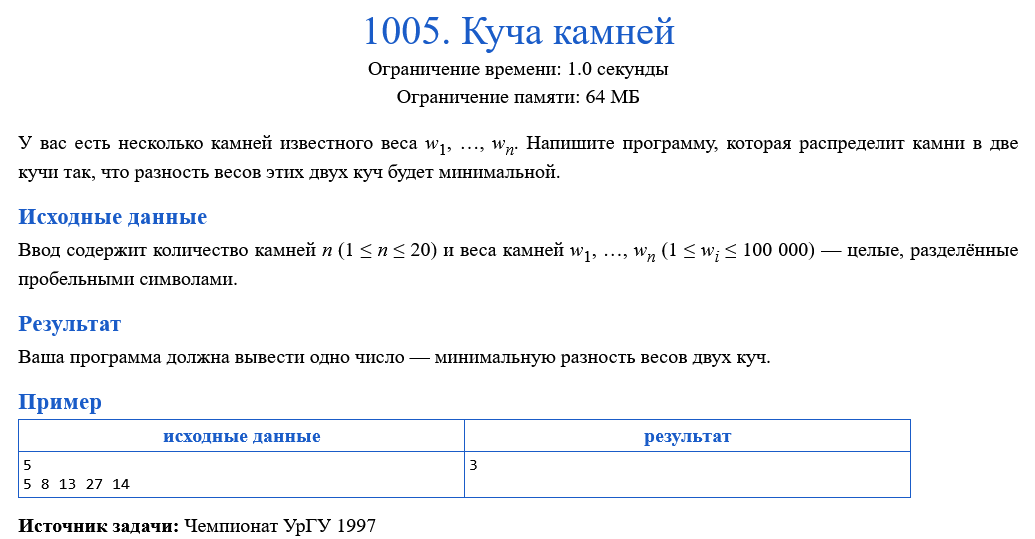
\includegraphics[width=1\linewidth]{pic/task_1005.png}}
\caption{Условие задачи 1005.}
\end{figure}

\subsection{Основная идея}
Заметим, что максимальное суммарное значение веса камней $20 \times 100000 = 2000000$, что на 3 порядка меньше, чем вмещает тип \textit{integer}, значит, мы работаем с относительно "небольшими" данными. К тому же, задача подобна \textit{Задаче о рюкзаке} ($NP-$полная задача, большие "рюкзаки" не решаются за разумное время), значит, мы можем точно решить данную задачу используя метод \textbf{\textit{перебора}} всех возможных вариантов распределения камней на 2 кучи.

\subsection{Краткое описание алгоритма}
\textbf{1. Входные данные:} $n$ -- количество камней $(1 \leq n \leq 20)$, $w_1, \, ... \, , \, w_n \, \, (1 \leq w_i \leq 100000)$ -- вес каждого камня.\\
\textbf{2.} Находим суммарный вес камней (\textit{full\_sum}).\\
\textbf{3.} Далее перебираем все возможные наборы. Воспользуемся свойством двоичной системы: пусть \textbf{1} == добавление камня в кучу, \textbf{0} == сумма камней в куче не меняется. Заметим, что нам достаточно перебрать только половину всех возможных наборов (остальные будут симметричными), поэтому итерации цикла будут от $0$ до $2^{n-1}$ с шагом 1. Для определения точного номера нужного камня введена дополнительная переменная \textit{iter\_numb}, использующаяся в последовательном вычислении остатков от деления номера итерации на 2.\\
\textbf{4.} Текущий минимум разности масс куч вычисляется с помощью стандартной функции \textit{std::min} языка \textit{C++}. \\
Пусть $s_1$ -- масса камней в первой куче, $s_2$ -- во второй, $S$ -- сумма всех камней. Формула для модуля текущей разницы масс: 
$$| s_2 - s_1| = | S - s_1 - s_1| = |S - 2 \cdot s_1|$$
\textbf{5. Выходные данные:} целое неотрицательное число -- минимальная разница масс куч.

\subsection{Структуры данных}
$std::vector<int>$ -- вектор из стандартной библиотеки \textit{C++} -- динамический массив.

\subsection{Листинг}

\begin{center}
\begin{lstlisting}[label=some-code,caption={Исходный код для 1005}]
#include <iostream>
#include <vector>
#include <cmath>
#include <algorithm>

int main() {
    int number;
    std::cin >> number;

    std::vector<int> stones_weights(number);

    int full_sum = 0;

    for (int i = 0; i < number; ++i) {
        std::cin >> stones_weights[i];
        full_sum += stones_weights[i];
    }

    int min = full_sum;

    for (int i = 0; i < pow(2, number - 1); ++i) {
        int cur = i;
        int iter_numb = 0;
        int first_sum = 0;
        while (cur != 0) {
            if (cur % 2 == 1) {
                first_sum += stones_weights[iter_numb];
            }
            cur = cur / 2;
            ++iter_numb;
        }
        min = std::min(min, std::abs(full_sum - 2 * first_sum));
    }
    printf("%d", min);

    return 0;
}


\end{lstlisting}
\end{center}

\subsection{Результат}
\begin{figure}[h]
\center{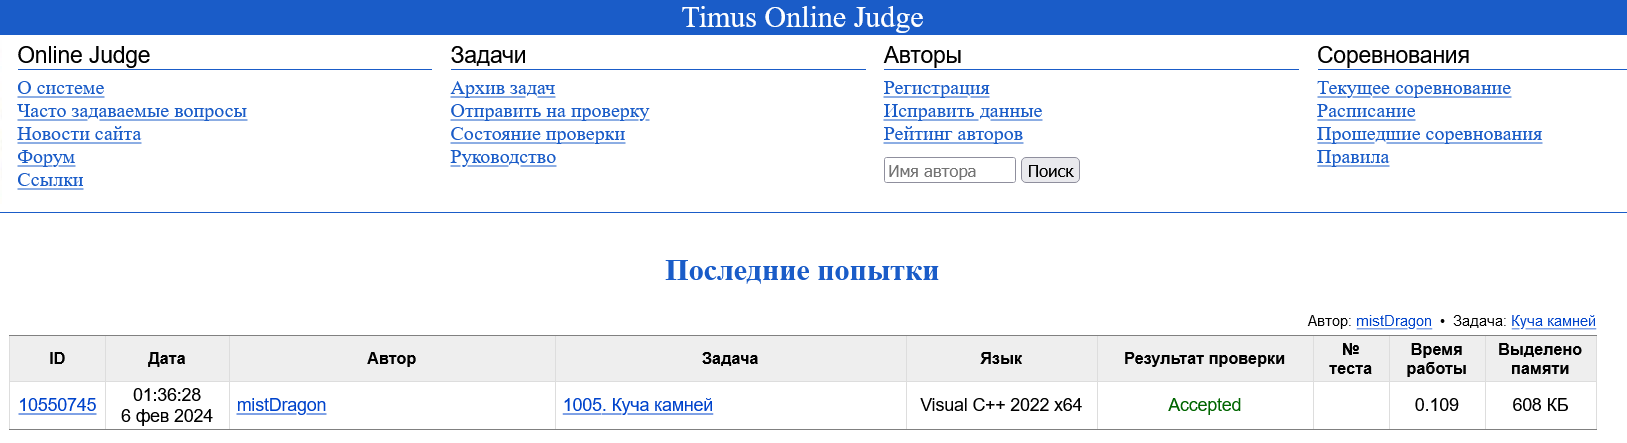
\includegraphics[width=0.9\linewidth]{pic/screen_1005.png}}
\caption{Результат отправки задачи 1005.}
\end{figure}


\newpage
\section{Задача 2025}

\begin{figure}[h]
\center{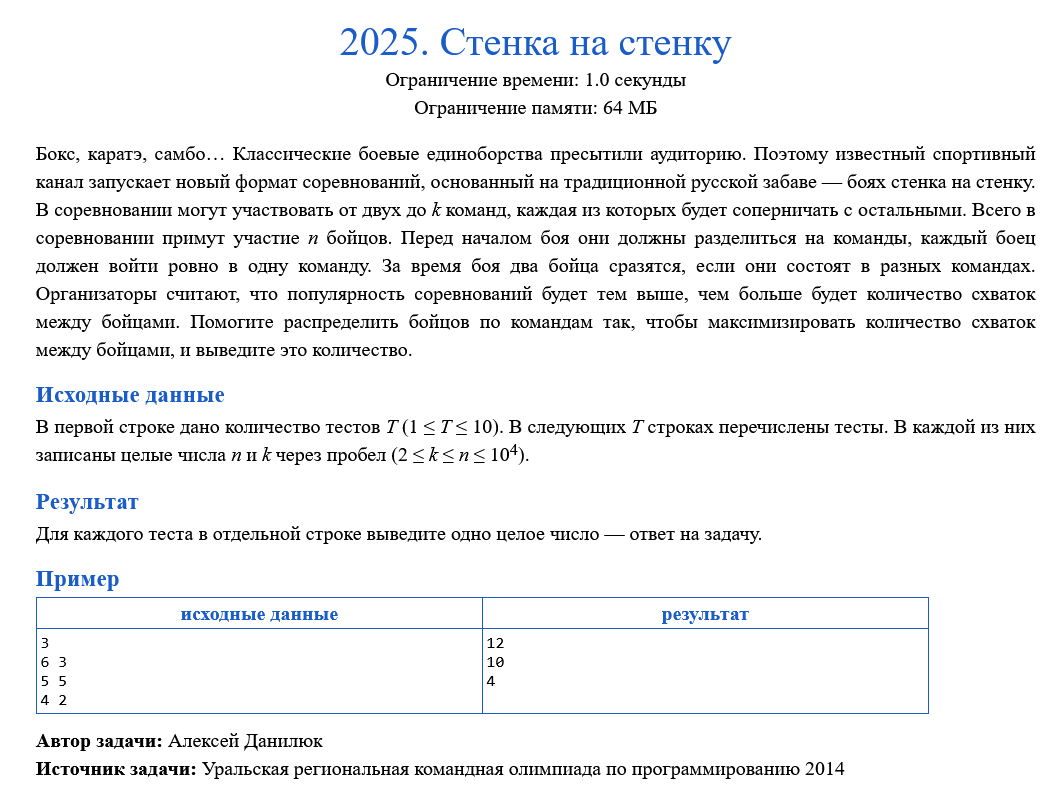
\includegraphics[width=0.94\linewidth]{pic/task_2025.png}}
\caption{Условие задачи 2025.}
\end{figure}


\subsection{Основная идея}
Для того, чтобы максимизировать число боев, необходимо, чтобы как можно меньше бойцов находились в одной команде. То есть, в идеале в каждой команде должно быть равное число бойцов, это выполнимо только в том случае, когда количество бойцов нацело делится на число команд. В случае ненулевого остатка от деления числа бойцов на число команд, оставшихся бойцов распределяем так же равномерно. Таким образом, число бойцов в каждой команде может различаться \textbf{не больше, чем на 1}.

\subsection{Краткое описание алгоритма}
\textbf{1. Входные данные:} $t$ -- количество тестов $(1 \leq t \leq 10)$,  в следующих $t$ строках перечислены тесты, в каждой из них 2 целые числа $n$ и $k$ $ (2 \leq k \leq n \leq 10^4)$.\\
\textbf{2.} Найдем среднее число бойцов в команде: для этого разделим общее количество бойцов на количество команд $medium\_in\_team = \frac{n}{k}$.\\
\textbf{3.} Найдем число бойцов пока не распределенных по командам как остаток от деления числа бойцов на количество команд: $extra\_fighters = n \%k$\\
\textbf{4.} Формула для подсчета числа боев: 
\begin{multline*}
F =medium\_in\_team \cdot (k - extra\_fighters) \cdot (n - medium\_in\_team) + \\
+ extra\_fighters \cdot (medium\_in\_team + 1) \cdot (n -( medium\_in\_team + 1))
\end{multline*}
Заметим, что сейчас симметричные бои учтены. Поэтому конечным результатом будет: $result = \frac{F}{2}$\\
\textbf{5. Выходные данные:} для каждого из $t$ наборов целое неотрицательное число -- максимальное количество боев.


\subsection{Листинг}

\begin{center}
\begin{lstlisting}[label=some-code,caption={Исходный код для 2025}]
#include <iostream>


int main() {
    int numb_test;
    std::cin >> numb_test;

    for (int i = 0; i < numb_test; ++i) {

        int fighters, teams;
        std::cin >> fighters;
        std::cin >> teams;

        int medium_in_team = fighters / teams;
        int extra_fighters = fighters % teams;
        int result = (medium_in_team * (teams - extra_fighters) * (fighters - medium_in_team) +
                      extra_fighters * (medium_in_team + 1) *
                      (fighters - medium_in_team - 1)) / 2;

        std::cout << result << std::endl;
    }
}

\end{lstlisting}
\end{center}

\subsection{Результат}
\begin{figure}[h]
\center{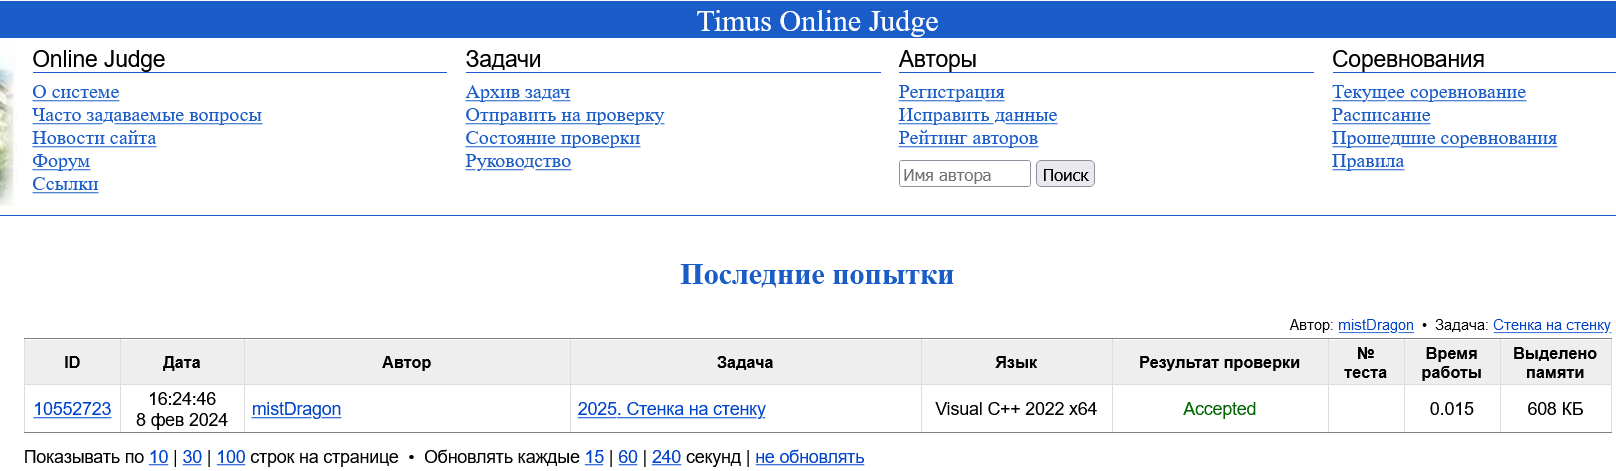
\includegraphics[width=1\linewidth]{pic/screen_2025.png}}
\caption{Результат отправки задачи 2025.}
\end{figure}

\newpage
\section{Задача 1155}

\begin{figure}[h]
\center{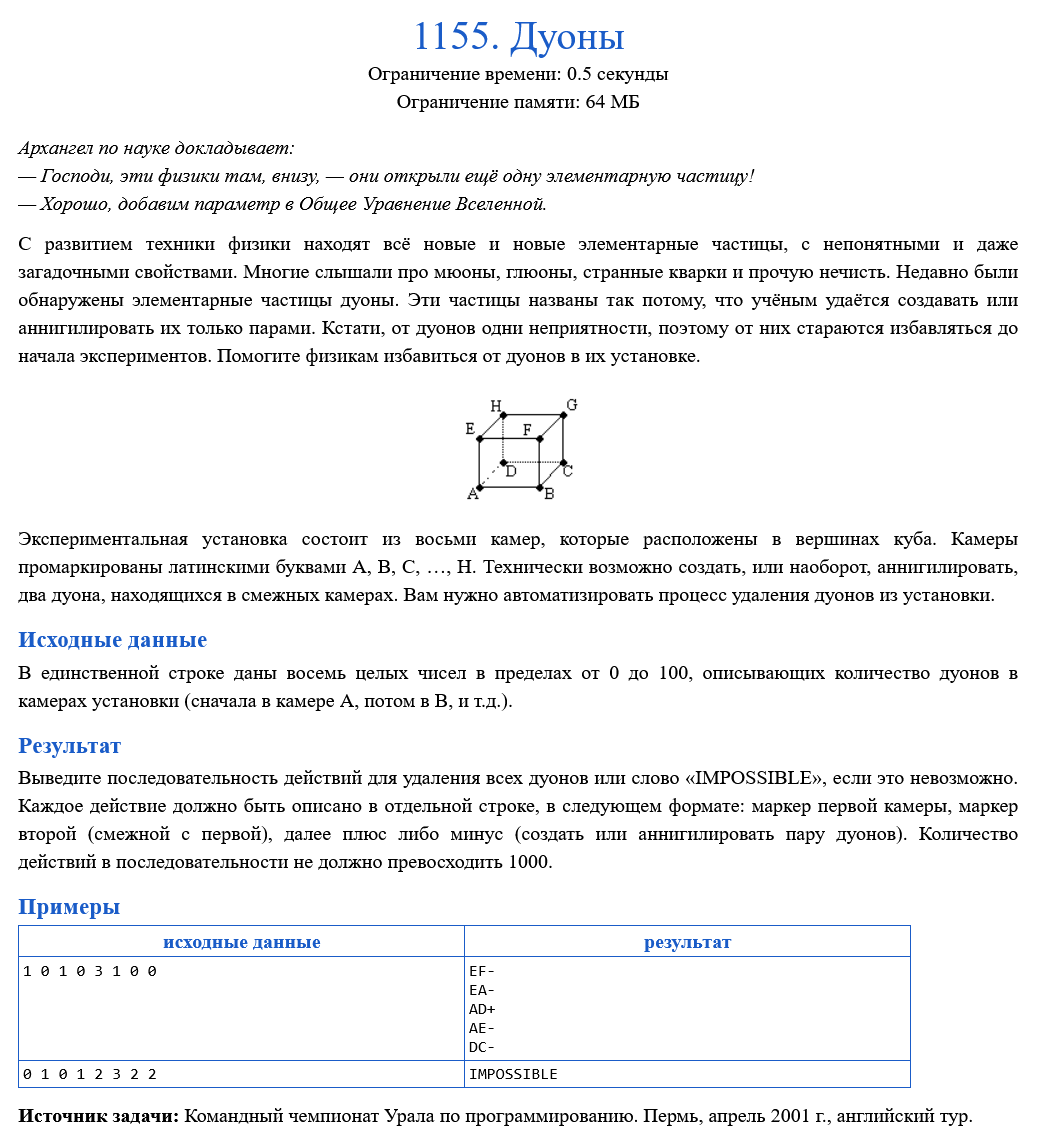
\includegraphics[width=0.9\linewidth]{pic/task_1155.png}}
\caption{Условие задачи 1155.}
\end{figure}

\subsection{Основная идея}
В начале проверим условие возможности аннигиляции всех дуонов куба: суммы дуонов на несмежных вершинах должны быть равны между собой. То есть $A + C + F + H = B + E + D + G$. Основная идея состоит в том, чтобы последовательно обнулять вершины, начиная с A, далее B,  D, E и G, обнуление этих вершин повлечет за собой обнуление и $C, F, H$, что следует из условия выполнения проверки перед началом выполнения алгоритма.

\subsection{Листинг}

\begin{center}
\begin{lstlisting}[label=some-code,caption={Исходный код для 1155}]
#include <iostream>
#include <vector>
#include <string>
#include <algorithm>

int cube[8];
std::vector<std::string> v_names = {"A", "B", "C", "D", "E", "F", "G", "H"};

void annihilate(int ind_1, int ind_2) {
    int min_numb = std::min(cube[ind_1], cube[ind_2]);

    for (int i = 0; i < min_numb; ++i) {
        std::cout << v_names[ind_1] + v_names[ind_2] + "-" << std::endl;
        --cube[ind_1];
        --cube[ind_2];
    }
}

void create(int ind_1, int ind_2, int cost) {

    for (int i = 0; i < cost; ++i) {
        std::cout << v_names[ind_1] + v_names[ind_2] + "+" << std::endl;
        ++cube[ind_1];
        ++cube[ind_2];
    }
}

int main() {
    int sum_of_all = 0;

    for (int i = 0; i < 8; ++i) {
        std::cin >> cube[i];
        sum_of_all += cube[i];
    }

    // checking the possibility of annihilating duons
    if ((cube[0] + cube[2] + cube[5] + cube[7]) != (cube[1] + cube[3] + cube[4] + cube[6])) {
        std::cout << "IMPOSSIBLE" << std::endl;
    } else {
        // take A and annihilate it using adjacent vertices
        annihilate(0, 1);
        annihilate(0, 3);
        annihilate(0, 4);
        // if after this vertex A (0) is not reset, we achieve one (paired with its adjacent vertex) from adjacent vertices to the value of A
        if (cube[0] > 0) {
            create(1, 2, cube[0]);
        }
        // here A goes to zero
        annihilate(0, 1);

        // take 2nd vertex B and annihilate with all adjacent vertices except zeroed A
        annihilate(1, 2);
        annihilate(1, 5);

        if (cube[1] > 0) {
            create(2, 6, cube[1]);
        }
        annihilate(1, 2);

        //  D goes to zero
        annihilate(3, 2);
        annihilate(3, 7);

        if (cube[3] > 0) {
            create(7, 6, cube[3]);
        }
        annihilate(3, 7);

        // E goes to zero
        annihilate(4, 5);
        annihilate(4, 7);

        if (cube[4] > 0) {
            create(7, 6, cube[4]);
        }
        annihilate(4, 7);

        //  G goes to zero
        annihilate(6, 2);
        annihilate(6, 5);
        annihilate(6, 7);

    }
}
\end{lstlisting}
\end{center}

\subsection{Результат}
\begin{figure}[h]
\center{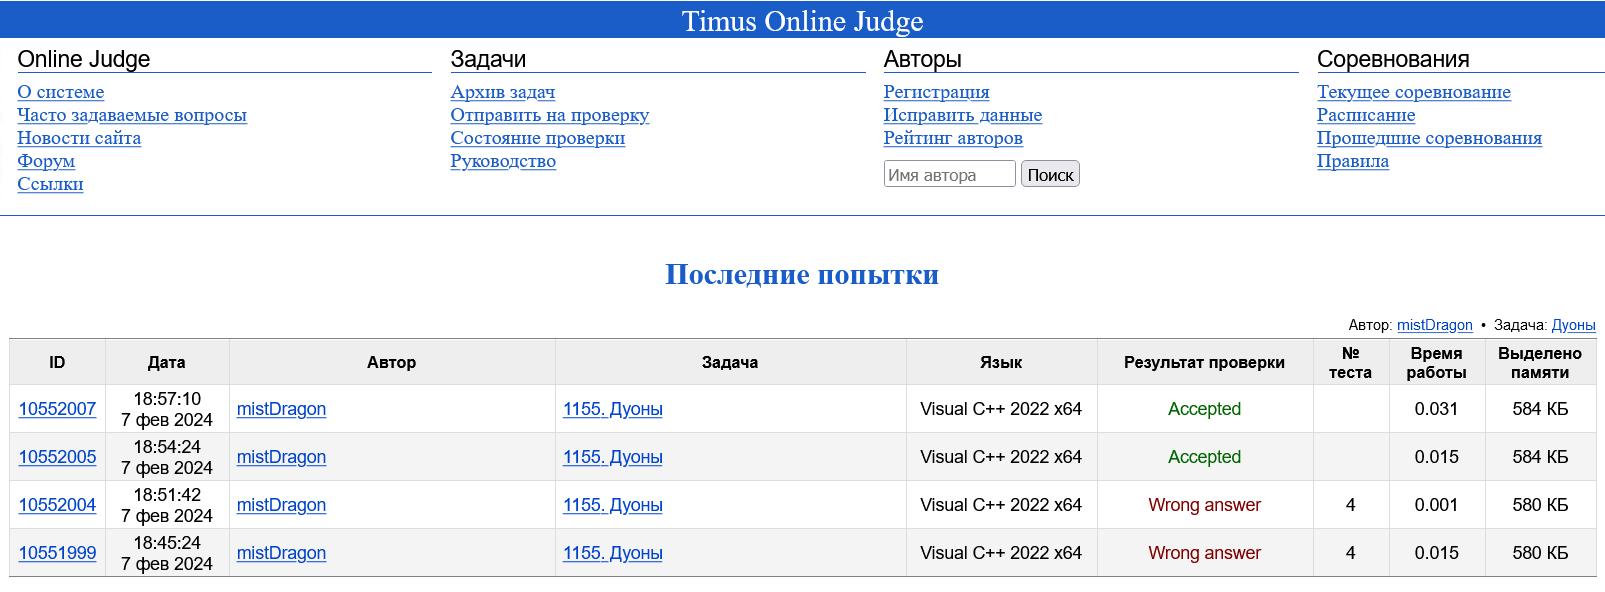
\includegraphics[width=1\linewidth]{pic/screen_1155.png}}
\caption{Результат отправки задачи 1155.}
\end{figure}


\newpage
\section{Вывод по работе}
В ходе выполнения данной лабораторной работы были оеализованы алгоритмы для решения задач $1005$, $2025$ и $1155$. Заметим, что они не содержат сложных структур данных.
\end{document}













